% !TEX program = pdflatex
% ------------------------------------------------------------
% ITKA2004 Databases & Data Management
% Lecture: Big Data Technologies (MapReduce + Hadoop) (90 min)
% Theme: metropolis (TikZ-only figures)
% Michael Emmerich, Professor of Intelligent Computing, PS Fellow
% Faculty of Information Technology, University of Jyväskylä
% ------------------------------------------------------------
\documentclass[10pt,aspectratio=169]{beamer}

\usetheme[
  progressbar=frametitle,
  numbering=fraction
]{metropolis}

% --- Packages
\usepackage[utf8]{inputenc}
\usepackage{amsmath,amssymb}
\usepackage{booktabs}
\usepackage{xcolor}
\usepackage{tikz}
\usetikzlibrary{positioning,arrows.meta,shapes.geometric,calc,fit}

% --- JYU-ish colors (adjust if you have official codes)
\definecolor{JYUblue}{HTML}{003A70}
\definecolor{JYUorange}{HTML}{FF6A00}

% --- Metropolis palette / accents
\setbeamercolor{palette primary}{bg=JYUblue, fg=white}
\setbeamercolor{frametitle}{bg=JYUblue!6, fg=JYUblue}
\setbeamercolor{progress bar}{fg=JYUorange, bg=JYUblue!20}
\setbeamercolor{structure}{fg=JYUblue}
\setbeamercolor{alerted text}{fg=JYUorange}
\setbeamercolor{title}{fg=JYUblue}
\setbeamercolor{subtitle}{fg=JYUblue!85}

% --- Blocks: blue for theory, orange for examples
\setbeamercolor{block title}{bg=JYUblue, fg=white}
\setbeamercolor{block body}{bg=JYUblue!5, fg=black}
\setbeamercolor{block title example}{bg=JYUorange, fg=white}
\setbeamercolor{block body example}{bg=JYUorange!10, fg=black}

% --- Theorem/definition styling
\setbeamertemplate{theorems}[numbered]
\newtheorem{definition}{Definition}
\newtheorem{theorem}{Theorem}
\newtheorem{remark}{Remark}
\newenvironment{examplebox}[1][Example]{\begin{exampleblock}{#1}}{\end{exampleblock}}

% ------------------------------------------------------------
% Footer (Metropolis)
% ------------------------------------------------------------
\setbeamertemplate{frame footer}{%
  \tiny Michael Emmerich (Professor of Intelligent Computing, PS Fellow)\hfill Databases Spring 2026\hfill Faculty of Information Technology, University of Jyväskylä%
}

% --- Metadata
\title{Databases and Data Management}
\subtitle{Big Data Technologies: MapReduce and Hadoop}
\author{Michael Emmerich (Professor of Intelligent Computing, PS Fellow)}
\institute{Faculty of Information Technology\\University of Jyväskylä}
\date{Spring 2026}

% --- Title graphic (TikZ-only)
\titlegraphic{%
  \begin{tikzpicture}[remember picture,overlay]
    \node[anchor=south east,opacity=0.10] at ([xshift=-2mm,yshift=2mm]current page.south east) {%
      \begin{tikzpicture}[scale=0.75]
        \draw[rounded corners=6pt,line width=2pt] (0,0) rectangle (5,3);
        \draw[line width=2pt] (0.6,2.4) -- (4.4,2.4);
        \node[text=JYUblue] at (2.5,1.55) {\Large MR};
        \node[text=JYUblue] at (2.5,0.95) {\large HDFS};
      \end{tikzpicture}
    };
  \end{tikzpicture}%
}

% --- Small helpers
\newcommand{\tinytable}[1]{{\scriptsize #1}}
\tikzset{
  box/.style={draw,rounded corners,align=center,inner sep=4pt},
  arr/.style={-Latex,thick},
  soft/.style={draw,rounded corners,fill=black!3,align=center,inner sep=4pt},
  nodebig/.style={draw,rounded corners,fill=JYUblue!6,align=center,inner sep=6pt}
}

\begin{document}

\maketitle

% ============================================================
\begin{frame}{Today (90 minutes)}
\begin{itemize}
  \item What is “Big Data” and why traditional DBMS struggle
  \item Hadoop ecosystem at a glance: HDFS + MapReduce (+ resource management)
  \item MapReduce programming model (map, shuffle/sort, reduce)
  \item MapReduce runtime: job submission, scheduling, execution
  \item Fault tolerance and the shuffle
  \item Achieving joins in MapReduce: major strategies
  \item When Hadoop/MapReduce is a good fit (and when not)
\end{itemize}
\end{frame}

\begin{frame}{Learning goals}
After this lecture you can:
\begin{enumerate}
  \item explain why “big data” needs distributed storage + compute
  \item describe HDFS (blocks, replication, NameNode/DataNodes) and scalability considerations
  \item describe the MapReduce dataflow and write simple MR pseudocode
  \item explain the runtime roles (JobTracker/TaskTracker) and what the shuffle does
  \item explain common failure modes and how MR recovers
  \item compare join strategies in MapReduce (reduce-side, map-side, partition, bucket, n-way)
\end{enumerate}
\end{frame}

\begin{frame}{Outline}
\tableofcontents
\end{frame}

% ============================================================
\section{Big Data: motivation and problem setting}

\begin{frame}{Big Data: the practical motivation}
\begin{itemize}
  \item Explosion of data from devices, sensors, web, social media, and enterprise systems.
  \item Not just “more rows”: also more \textbf{variety}, higher \textbf{velocity}, and distributed sources.
  \item Organizations want analytics:
  \begin{itemize}
    \item \textbf{descriptive} (what happened?)
    \item \textbf{predictive} (what will happen?)
    \item \textbf{prescriptive} (what should we do?)
  \end{itemize}
\end{itemize}
\end{frame}

\begin{frame}{Why traditional DBMS alone may not scale}
\begin{itemize}
  \item Datasets so large that:
  \begin{itemize}
    \item storing on one machine is too costly or impossible
    \item processing needs parallelism across many machines
  \end{itemize}
  \item Need a stack that supports:
  \begin{itemize}
    \item distributed file storage (fault-tolerant, scalable)
    \item distributed batch computation (parallel, data-local)
  \end{itemize}
  \item MapReduce + Hadoop emerged as a pragmatic approach for large-scale batch analytics.
\end{itemize}
\end{frame}

\begin{frame}{Concept map (where MapReduce fits)}
\centering
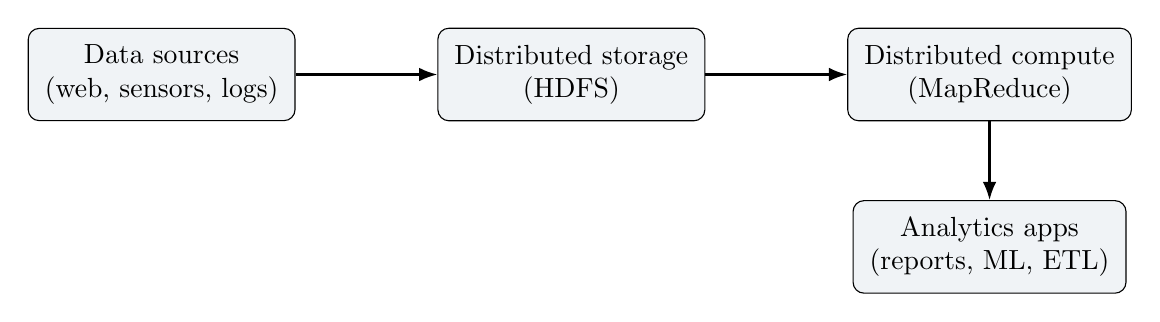
\begin{tikzpicture}[node distance=10mm]
\node[nodebig] (data) {Data sources\\(web, sensors, logs)};
\node[nodebig, right=18mm of data] (store) {Distributed storage\\(HDFS)};
\node[nodebig, right=18mm of store] (compute) {Distributed compute\\(MapReduce)};
\node[nodebig, below=10mm of compute] (apps) {Analytics apps\\(reports, ML, ETL)};
\draw[arr] (data) -- (store);
\draw[arr] (store) -- (compute);
\draw[arr] (compute) -- (apps);
\end{tikzpicture}
\end{frame}

% ============================================================
\section{Hadoop ecosystem overview}

\begin{frame}{Hadoop in one picture}
\centering
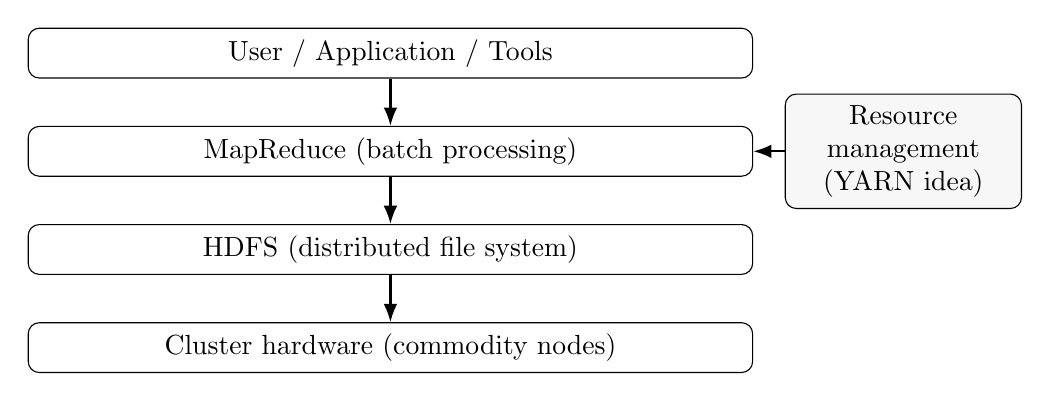
\begin{tikzpicture}[node distance=8mm]
\node[box, minimum width=9.2cm] (user) {User / Application / Tools};
\node[box, below=6mm of user, minimum width=9.2cm] (mr) {MapReduce (batch processing)};
\node[box, below=6mm of mr, minimum width=9.2cm] (hdfs) {HDFS (distributed file system)};
\node[box, below=6mm of hdfs, minimum width=9.2cm] (cluster) {Cluster hardware (commodity nodes)};

\draw[arr] (user) -- (mr);
\draw[arr] (mr) -- (hdfs);
\draw[arr] (hdfs) -- (cluster);

\node[soft, right=4mm of mr, minimum width=3.0cm] (rm) {Resource\\management\\(YARN idea)};
\draw[arr] (rm.west) -- (mr.east);
\end{tikzpicture}
\end{frame}

\begin{frame}{HDFS: what it provides}
\begin{itemize}
  \item File system for huge files, split into large \textbf{blocks}
  \item \textbf{Replication} of blocks for fault tolerance
  \item Supports \textbf{streaming reads/writes} (batch-friendly)
  \item Enables \textbf{data locality}: run computation near the data blocks
\end{itemize}
\end{frame}

\begin{frame}{HDFS architecture (NameNode and DataNodes)}
\centering
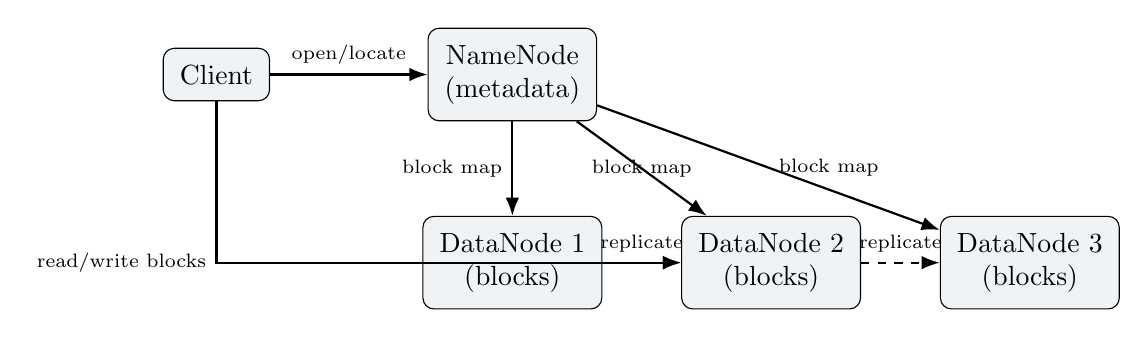
\begin{tikzpicture}[node distance=10mm]
\node[nodebig] (client) {Client};
\node[nodebig, right=20mm of client] (nn) {NameNode\\(metadata)};
\node[nodebig, below=12mm of nn] (dn1) {DataNode 1\\(blocks)};
\node[nodebig, right=10mm of dn1] (dn2) {DataNode 2\\(blocks)};
\node[nodebig, right=10mm of dn2] (dn3) {DataNode 3\\(blocks)};

\draw[arr] (client) -- node[above, font=\scriptsize]{open/locate} (nn);
\draw[arr] (client) |- node[left, font=\scriptsize]{read/write blocks} (dn2);

\draw[arr] (nn) -- node[left, font=\scriptsize]{block map} (dn1);
\draw[arr] (nn) -- node[font=\scriptsize]{block map} (dn2);
\draw[arr] (nn) -- node[right, font=\scriptsize]{block map} (dn3);

\draw[arr, dashed] (dn1) -- node[above, font=\scriptsize]{replicate} (dn2);
\draw[arr, dashed] (dn2) -- node[above, font=\scriptsize]{replicate} (dn3);
\end{tikzpicture}
\end{frame}

\begin{frame}{HDFS scalability: what becomes expensive}
\begin{itemize}
  \item NameNode holds metadata (blocks, file namespace).
  \item Many small files can be problematic (metadata overhead).
  \item Replication and block reports create background traffic.
  \item Tuning: block size, replication factor, number of DataNodes.
\end{itemize}
\end{frame}

% ============================================================
\section{MapReduce programming model}

\begin{frame}{MapReduce: key idea}
\begin{definition}[MapReduce (high-level)]
A batch processing model where:
\begin{itemize}
  \item \textbf{Map} transforms input records into intermediate \((k,v)\) pairs
  \item \textbf{Shuffle/Sort} groups all values by key
  \item \textbf{Reduce} aggregates per-key groups into output records
\end{itemize}
\end{definition}
\end{frame}

\begin{frame}{MapReduce dataflow (classic pipeline)}
\centering
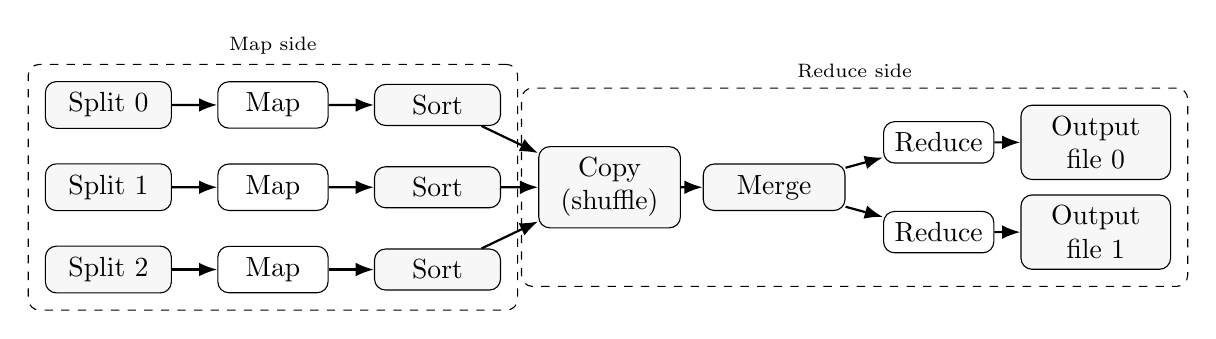
\begin{tikzpicture}[x=1cm,y=1cm,scale=0.95]
\node[soft, minimum width=1.6cm] (in0) at (0,3.0) {Split 0};
\node[soft, minimum width=1.6cm] (in1) at (0,1.9) {Split 1};
\node[soft, minimum width=1.6cm] (in2) at (0,0.8) {Split 2};

\node[box, minimum width=1.4cm] (m0) at (2.2,3.0) {Map};
\node[box, minimum width=1.4cm] (m1) at (2.2,1.9) {Map};
\node[box, minimum width=1.4cm] (m2) at (2.2,0.8) {Map};

\node[soft, minimum width=1.6cm] (s0) at (4.4,3.0) {Sort};
\node[soft, minimum width=1.6cm] (s1) at (4.4,1.9) {Sort};
\node[soft, minimum width=1.6cm] (s2) at (4.4,0.8) {Sort};

\node[soft, minimum width=1.8cm] (copy) at (6.7,1.9) {Copy\\(shuffle)};
\node[soft, minimum width=1.8cm] (merge) at (8.9,1.9) {Merge};

\node[box, minimum width=1.4cm] (r0) at (11.1,2.5) {Reduce};
\node[box, minimum width=1.4cm] (r1) at (11.1,1.3) {Reduce};

\node[soft, minimum width=1.9cm] (out0) at (13.2,2.5) {Output\\file 0};
\node[soft, minimum width=1.9cm] (out1) at (13.2,1.3) {Output\\file 1};

\draw[arr] (in0) -- (m0);
\draw[arr] (in1) -- (m1);
\draw[arr] (in2) -- (m2);

\draw[arr] (m0) -- (s0);
\draw[arr] (m1) -- (s1);
\draw[arr] (m2) -- (s2);

\draw[arr] (s0) -- (copy);
\draw[arr] (s1) -- (copy);
\draw[arr] (s2) -- (copy);

\draw[arr] (copy) -- (merge);
\draw[arr] (merge) -- (r0);
\draw[arr] (merge) -- (r1);

\draw[arr] (r0) -- (out0);
\draw[arr] (r1) -- (out1);

\node[draw,dashed,rounded corners,fit=(in0) (in2) (m0) (m2) (s0) (s2), inner sep=6pt,label={[font=\scriptsize]above:Map side}] {};
\node[draw,dashed,rounded corners,fit=(copy) (merge) (r0) (r1) (out0) (out1), inner sep=6pt,label={[font=\scriptsize]above:Reduce side}] {};
\end{tikzpicture}
\end{frame}

\begin{frame}{Example: Word Count (pseudocode)}
\begin{examplebox}[Map and Reduce idea]
\begin{itemize}
  \item \textbf{Map}: for each word emit \((word,1)\)
  \item \textbf{Reduce}: sum the counts for each word
\end{itemize}
\end{examplebox}

\scriptsize
\[
\texttt{map(key, value): for each word w in value: emit(w, 1)}
\]
\[
\texttt{reduce(key=w, values=[1,1,1,...]): emit(w, sum(values))}
\]
\end{frame}

\begin{frame}{More MapReduce “patterns”}
Typical MapReduce applications include:
\begin{itemize}
  \item distributed grep (pattern match lines)
  \item reverse web-link graph (aggregate inbound links)
  \item inverted index (word $\rightarrow$ list of documents)
\end{itemize}
\begin{examplebox}[Inverted index sketch]
\textbf{Map}: emit \((word, docid)\) for each word occurrence\\
\textbf{Reduce}: emit \((word, \{docid\}\_{\text{unique}})\)
\end{examplebox}
\end{frame}

% ============================================================
\section{MapReduce runtime: jobs, scheduling, shuffle}

\begin{frame}{MapReduce runtime (v1 view)}
\begin{itemize}
  \item A job consists of:
  \begin{itemize}
    \item map tasks
    \item reduce tasks
    \item configuration (input, output, number of reducers, etc.)
  \end{itemize}
  \item Classic Hadoop v1 roles:
  \begin{itemize}
    \item \textbf{JobTracker} (master)
    \item \textbf{TaskTrackers} (workers)
  \end{itemize}
\end{itemize}
\end{frame}

\begin{frame}{JobTracker and TaskTracker (roles)}
\centering
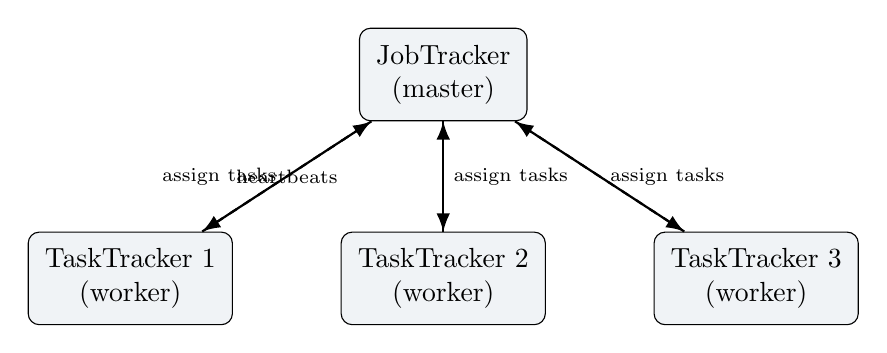
\begin{tikzpicture}[node distance=10mm]
\node[nodebig] (jt) {JobTracker\\(master)};
\node[nodebig, below left=14mm and 16mm of jt] (tt1) {TaskTracker 1\\(worker)};
\node[nodebig, below=14mm of jt] (tt2) {TaskTracker 2\\(worker)};
\node[nodebig, below right=14mm and 16mm of jt] (tt3) {TaskTracker 3\\(worker)};

\draw[arr] (jt) -- node[left, font=\scriptsize]{assign tasks} (tt1);
\draw[arr] (jt) -- node[right, font=\scriptsize]{assign tasks} (tt3);
\draw[arr] (jt) -- node[right, font=\scriptsize]{assign tasks} (tt2);

\draw[arr, dashed] (tt1) -- node[font=\scriptsize]{heartbeats} (jt);
\draw[arr, dashed] (tt2) -- (jt);
\draw[arr, dashed] (tt3) -- (jt);
\end{tikzpicture}
\end{frame}

\begin{frame}{Lifecycle of a MapReduce job}
\begin{columns}[T,onlytextwidth]
\column{0.52\textwidth}
\begin{block}{High-level steps}
\begin{enumerate}
  \item Job submission (client $\rightarrow$ master)
  \item Task assignment (map tasks, then reduce tasks)
  \item Task execution on worker nodes
  \item Job completion (commit outputs)
\end{enumerate}
\end{block}

\column{0.48\textwidth}
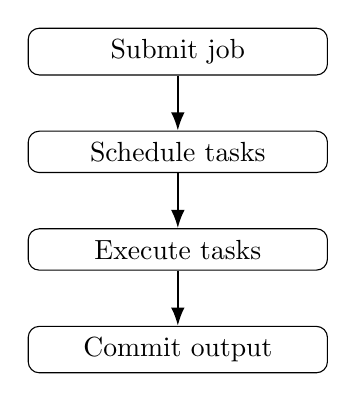
\begin{tikzpicture}[node distance=7mm]
\node[box, minimum width=3.8cm] (sub) {Submit job};
\node[box, below=of sub, minimum width=3.8cm] (sched) {Schedule tasks};
\node[box, below=of sched, minimum width=3.8cm] (exec) {Execute tasks};
\node[box, below=of exec, minimum width=3.8cm] (commit) {Commit output};
\draw[arr] (sub) -- (sched);
\draw[arr] (sched) -- (exec);
\draw[arr] (exec) -- (commit);
\end{tikzpicture}
\end{columns}
\end{frame}

\begin{frame}{The shuffle (why it matters)}
\begin{itemize}
  \item The shuffle ensures: all values for a key meet at the same reducer.
  \item Implemented via:
  \begin{itemize}
    \item partitioner (assigns keys to reducers)
    \item sorting/grouping (by key)
    \item merging intermediate files
    \item optional combiner (local pre-aggregation)
  \end{itemize}
\end{itemize}

\begin{examplebox}[Rule of thumb]
Use a \textbf{combiner} when your reduce operation is associative/commutative (e.g., sum, count).
\end{examplebox}
\end{frame}

\begin{frame}{Partitioner, combiner, and sort (concept diagram)}
\centering
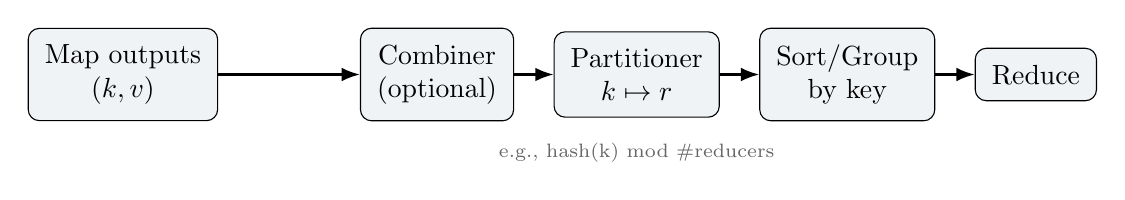
\begin{tikzpicture}[node distance=4mm]
\node[nodebig] (map) {Map outputs\\\((k,v)\)};
\node[nodebig, right=18mm of map] (comb) {Combiner\\(optional)};
\node[nodebig, right=5mm of comb] (part) {Partitioner\\\(k\mapsto r\)};
\node[nodebig, right=5mm of part] (sort) {Sort/Group\\by key};
\node[nodebig, right=5mm of sort] (red) {Reduce};

\draw[arr] (map) -- (comb);
\draw[arr] (comb) -- (part);
\draw[arr] (part) -- (sort);
\draw[arr] (sort) -- (red);

\node[font=\scriptsize, text=black!60, below=2mm of part] {e.g., hash(k) mod \#reducers};
\end{tikzpicture}
\end{frame}

% ============================================================
\section{Fault tolerance}

\begin{frame}{Fault tolerance in MapReduce (typical failures)}
\begin{itemize}
  \item Task failure: code exception or machine crash
  \item Worker failure: TaskTracker goes down or disconnects
  \item Master failure: JobTracker as a single point (classic Hadoop v1 limitation)
\end{itemize}
\begin{examplebox}[Recovery idea]
Re-execute failed tasks (map/reduce are deterministic given inputs).
\end{examplebox}
\end{frame}

\begin{frame}{Determinism and output commit}
\begin{itemize}
  \item If map/reduce are deterministic, re-running tasks yields consistent results.
  \item Output commit protocol helps avoid duplicated final results:
  \begin{itemize}
    \item tasks write to temporary locations
    \item successful completion commits final output
  \end{itemize}
\end{itemize}
\end{frame}

% ============================================================
\section{Joins in MapReduce}

\begin{frame}{Why joins are hard in MapReduce}
\begin{itemize}
  \item Joins are central in relational databases.
  \item In MapReduce, join requires co-locating matching keys across distributed data.
  \item Strategy depends on sizes, partitioning, and whether one side is “small”.
\end{itemize}
\end{frame}

\begin{frame}{Reduce-side join (general, but expensive shuffle)}
\begin{block}{Idea}
Tag tuples with their source relation, shuffle by join key, reduce joins matching groups.
\end{block}

\begin{columns}[T,onlytextwidth]
\column{0.55\textwidth}
\begin{examplebox}[Map outputs]
For join \(R(A,B)\Join S(B,C)\) on \(B\):
\[
\texttt{emit}(B,\langle R,A\rangle)\quad\text{and}\quad \texttt{emit}(B,\langle S,C\rangle)
\]
\end{examplebox}
\begin{examplebox}[Reduce]
For each \(B\): output all combinations of matching \(R\)-tuples and \(S\)-tuples.
\end{examplebox}

\column{0.45\textwidth}
\centering
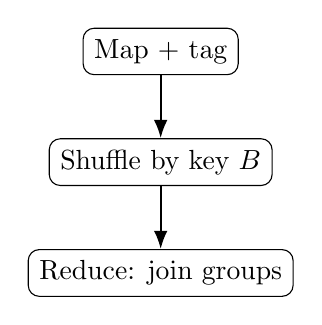
\begin{tikzpicture}[node distance=8mm]
\node[box] (m) {Map + tag};
\node[box, below=of m] (sh) {Shuffle by key \(B\)};
\node[box, below=of sh] (r) {Reduce: join groups};
\draw[arr] (m) -- (sh);
\draw[arr] (sh) -- (r);
\end{tikzpicture}
\end{columns}
\end{frame}

\begin{frame}{Map-side join (when one side is small)}
\begin{block}{Idea}
Load small relation into memory at mappers; stream over large relation.
\end{block}
\begin{itemize}
  \item Works when one input is small enough to broadcast (e.g., a dimension table).
  \item Avoids heavy shuffle of both sides.
\end{itemize}

\begin{examplebox}[Concept]
Mapper reads \(S\) into hash table keyed by join key; for each \(r\in R\), probe and emit joined results.
\end{examplebox}
\end{frame}

\begin{frame}{Partition join (both sides pre-partitioned)}
\begin{block}{Idea}
If \(R\) and \(S\) are partitioned by join key into matching partitions, each reducer joins one partition pair.
\end{block}

\centering
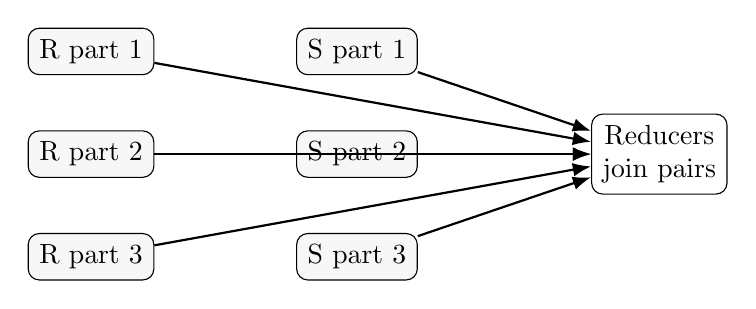
\begin{tikzpicture}[node distance=7mm]
\node[soft] (r1) {R part 1};
\node[soft, below=of r1] (r2) {R part 2};
\node[soft, below=of r2] (r3) {R part 3};

\node[soft, right=18mm of r2] (s2) {S part 2};
\node[soft, above=of s2] (s1) {S part 1};
\node[soft, below=of s2] (s3) {S part 3};

\node[box, right=22mm of s2] (red) {Reducers\\join pairs};

\draw[arr] (r1) -- (red);
\draw[arr] (r2) -- (red);
\draw[arr] (r3) -- (red);
\draw[arr] (s1) -- (red);
\draw[arr] (s2) -- (red);
\draw[arr] (s3) -- (red);
\end{tikzpicture}
\end{frame}

\begin{frame}{Bucket join (hash buckets aligned)}
\begin{itemize}
  \item Hash-assign tuples into buckets on the join key.
  \item Join corresponding buckets (bucket 0 with bucket 0, etc.).
  \item Similar spirit to partition join; useful when data is organized accordingly.
\end{itemize}
\end{frame}

\begin{frame}{N-way map-side join (star schema intuition)}
\begin{itemize}
  \item One large fact table \(R\), several small dimension tables \(S_1,\dots,S_k\).
  \item Load hash tables for small dimensions into each mapper.
  \item Stream fact tuples and join locally in memory.
\end{itemize}
\begin{examplebox}[When it works]
Dimension tables must be small enough; mapper memory must suffice.
\end{examplebox}
\end{frame}

\begin{frame}{Join strategy cheat-sheet}
\begin{tabular}{@{}p{3.2cm}p{5.3cm}p{4.3cm}@{}}
\toprule
\textbf{Strategy} & \textbf{When good} & \textbf{Main cost} \\
\midrule
Reduce-side join & general case & large shuffle/sort \\
Map-side join & one side small & broadcast + memory \\
Partition/Bucket join & both sides aligned on key & preprocessing/constraints \\
N-way map-side join & fact + small dimensions & memory + distribution \\
\bottomrule
\end{tabular}
\end{frame}

% ============================================================
\section{Discussion}

\begin{frame}{Limits of MapReduce}
\begin{itemize}
  \item Great for batch ETL and large scans/aggregations.
  \item Not ideal for:
  \begin{itemize}
    \item low-latency interactive queries
    \item iterative ML algorithms (many passes over data)
    \item complex workflows needing fine-grained scheduling
  \end{itemize}
  \item Later ecosystems add higher-level layers and in-memory engines (e.g., Spark).
\end{itemize}
\end{frame}

\begin{frame}{Where this fits in the course}
\begin{itemize}
  \item Relational algebra + SQL explain \emph{what} queries mean.
  \item Query optimization explains \emph{how} to execute efficiently.
  \item MapReduce is an operational execution model for large-scale batch processing.
  \item Join strategies here connect back to join semantics and execution plans.
\end{itemize}
\end{frame}

% ============================================================
\section{Wrap-up}

\begin{frame}{Recap}
\begin{itemize}
  \item Big data motivates distributed storage + compute.
  \item HDFS: blocks, replication, NameNode/DataNodes, locality.
  \item MapReduce: map $\rightarrow$ shuffle/sort $\rightarrow$ reduce; key/value grouping.
  \item Runtime: job submission, scheduling, execution, shuffle; fault tolerance via re-execution.
  \item Joins in MR: reduce-side, map-side, partition/bucket, n-way variants.
\end{itemize}
\end{frame}

\begin{frame}{What to do before next lecture}
\begin{itemize}
  \item Practice: write MR pseudocode for:
  \begin{itemize}
    \item distributed grep
    \item inverted index
    \item reduce-side join \(R(A,B)\Join S(B,C)\)
  \end{itemize}
  \item Think: when would you prefer SQL-on-distributed-systems vs raw MapReduce?
\end{itemize}
\end{frame}

\begin{frame}{Q\&A}
\begin{itemize}
  \item Concept questions (HDFS, shuffle, joins)
  \item Practical questions (why shuffle dominates, when mappers need memory)
  \item Course connections (RA/SQL vs MR)
\end{itemize}
\end{frame}

\end{document}